\subsection{Prism design}
\label{prism}
Prism is quite important after the receiver's second parabolic to filter out all the noisy light except wavelength at 472[nm] to 474[nm]. The prism design contains glass material, the prism angle and incoming light angle. The general prism looks like:
\begin{figure}[ht!]
\centering
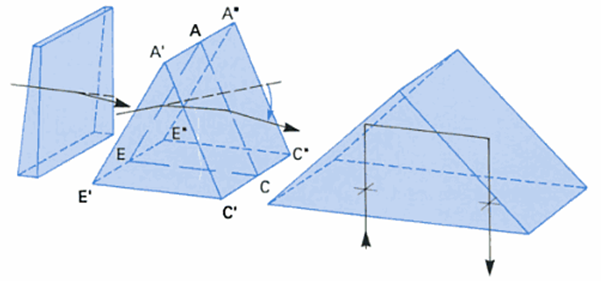
\includegraphics[scale = 1]{chapters/img/prism3D.png}
\caption{Prism in 3D}
\label{fig:prism3D}
\end{figure} 
\begin{figure}[ht!]
\centering
\includegraphics[scale = 1]{chapters/img/prism2D.png}
\caption{Prism configuration in 2D}
\label{fig:prism2D}
\end{figure} 
In figure \ref{prism2D} on page \ref{prism2D}, the outgoing angle $\epsilon$ can be calculated using the formula:

The main key requirement to design the prism is to maximize the 
